\documentclass[]{politex}
% ========== Opções ==========
% pnumromarab - Numeração de páginas usando algarismos romanos na parte pré-textual e arábicos na parte textual
% abnttoc - Forçar paginação no sumário conforme ABNT (inclui "p." na frente das páginas)
% normalnum - Numeração contínua de figuras e tabelas 
%	(caso contrário, a numeração é reiniciada a cada capítulo)
% draftprint - Ajusta as margens para impressão de rascunhos
%	(reduz a margem interna)
% twosideprint - Ajusta as margens para impressão frente e verso
% capsec - Forçar letras maiúsculas no título das seções
% espacosimples - Documento usando espaçamento simples
% espacoduplo - Documento usando espaçamento duplo
%	(o padrão é usar espaçamento 1.5)
% times - Tenta usar a fonte Times New Roman para o corpo do texto
% noindentfirst - Não indenta o primeiro parágrafo dos capítulos/seções


% ========== Packages ==========
\usepackage[utf8]{inputenc}
\usepackage{amsmath,amsthm,amsfonts,amssymb}
\usepackage{graphicx,cite,enumerate}


% ========== Language options ==========
\usepackage[brazil]{babel}
%\usepackage[english]{babel}


% ========== ABNT (requer ABNTeX 2) ==========
%	http://www.ctan.org/tex-archive/macros/latex/contrib/abntex2
\usepackage[num, abnt-etal-list=0]{abntex2cite}

% Forçar o abntex2 a usar [ ] nas referências ao invés de ( )
%\citebrackets{[}{]}


% ========== Lorem ipsum ==========
\usepackage{blindtext}



% ========== Opções do documento ==========
% Título
\titulo{Computação em Nuvem: Introdução}

% Para múltiplos autores (TCC)
\autor{Daniel Norio Takasu Rebelo\\%
    Lucas Arthur Felgueiras\\%
		Luiz Gustavo dos Santos\\%
		Victor França Ferreira}

% Orientador / Coorientador
\orientador{Profª. Drª. Selma Shin Shimizu Melnikoff}
% \coorientador{Nome do coorientador (opcional)}

% Tipo de documento
\trabalhoGenerico{Engenharia de Sistemas}
%\tcc{Engenharia de Computação}
%\dissertacao{Engenharia de Computação}
%\teseDOC{Engenharia Elétrica}
%\teseLD
%\memorialLD

% Departamento e área de concentração
\departamento{Engenharia de Computação e Sistemas Digitais}
\areaConcentracao{Engenharia de Sistemas}

% Local
\local{São Paulo}

% Ano
\data{2018}

\begin{document}
% ========== Capa e folhas de rosto ==========
\capa
\falsafolhaderosto
\folhaderosto


% ========== Folha de assinaturas (opcional) ==========
%\begin{folhadeaprovacao}
%	\assinatura{Prof.\ X}
%	\assinatura{Prof.\ Y}
%	\assinatura{Prof.\ Z}
%\end{folhadeaprovacao}


% ========== Ficha catalográfica ==========
% Fazer solicitação no site:
%	http://www.poli.usp.br/en/bibliotecas/servicos/catalogacao-na-publicacao.html


% ========== Dedicatória (opcional) ==========
% \dedicatoria{Dedicatória}


% ========== Agradecimentos ==========
% \begin{agradecimentos}

% Thanks...

% \end{agradecimentos}


% ========== Epígrafe (opcional) ==========
% \epigrafe{%
% 	\emph{``Epígrafe''}
% 	\begin{flushright}
% 		-{}- Autor
% 	\end{flushright}
% }


% ========== Resumo ==========
\begin{resumo}
A tecnologia de computação em nuvem é uma tendência para as novas aplicações do mundo. Grandes empresas estão migrando suas estruturas para a nuvem, outras constroem ambientes para abrigar essas novas aplicações. O objetivo do trabalho consiste em compreender melhor como funciona essas tecnologias, sua motivação e as principais opções disponíveis no mercado para uso.
%
\\[3\baselineskip]
%
\textbf{Palavras-Chave} -- Nuvem, Arquitetura, Computação, Engenharia, Programa.
\end{resumo}


% ========== Abstract ==========
\begin{abstract}
Cloud computing technology is a trend for new applications around the world. Large companies are migrating their structures to the cloud, others build environments to house these new applications. The objective of the work is to better understand how these technologies work, their motivation and the main options available in the market to use.
%
\\[3\baselineskip]
%
\textbf{Keywords} -- Cloud, Architecture, Computing, Enginnering, Software.
\end{abstract}


% ========== Listas (opcional) ==========
\listadefiguras
\listadetabelas

% ========== Listas definidas pelo usuário (opcional) ==========
% \begin{pretextualsection}{Lista de símbolos}

% Lista de símbolos...

% \end{pretextualsection}

% ========== Sumário ==========
\sumario

% ========== Elementos textuais ==========

\part{Introdução}

\chapter{Objetivo}
\capepigrafe[0.5\textwidth]{First to mind when asked what 'the cloud' is, a majority respond it’s either an actual cloud, the sky, or something related to weather.}{Citrix Cloud Survey Guide\cite{quotes}}

Com o desenvolvimento da computação, novos programas foram criados, cada vez mais consumindo recursos e sendo hospedados em máquinas pessoais ou dedicadas, porém sem um gerenciamento inteligente de toda a infraestrutura. Além disso, houve a nítida migração de programas \textbf{distribuídos} pela internet para programas que \textbf{rodem} na internet.

\begin{figure}[h!]
  \centering
  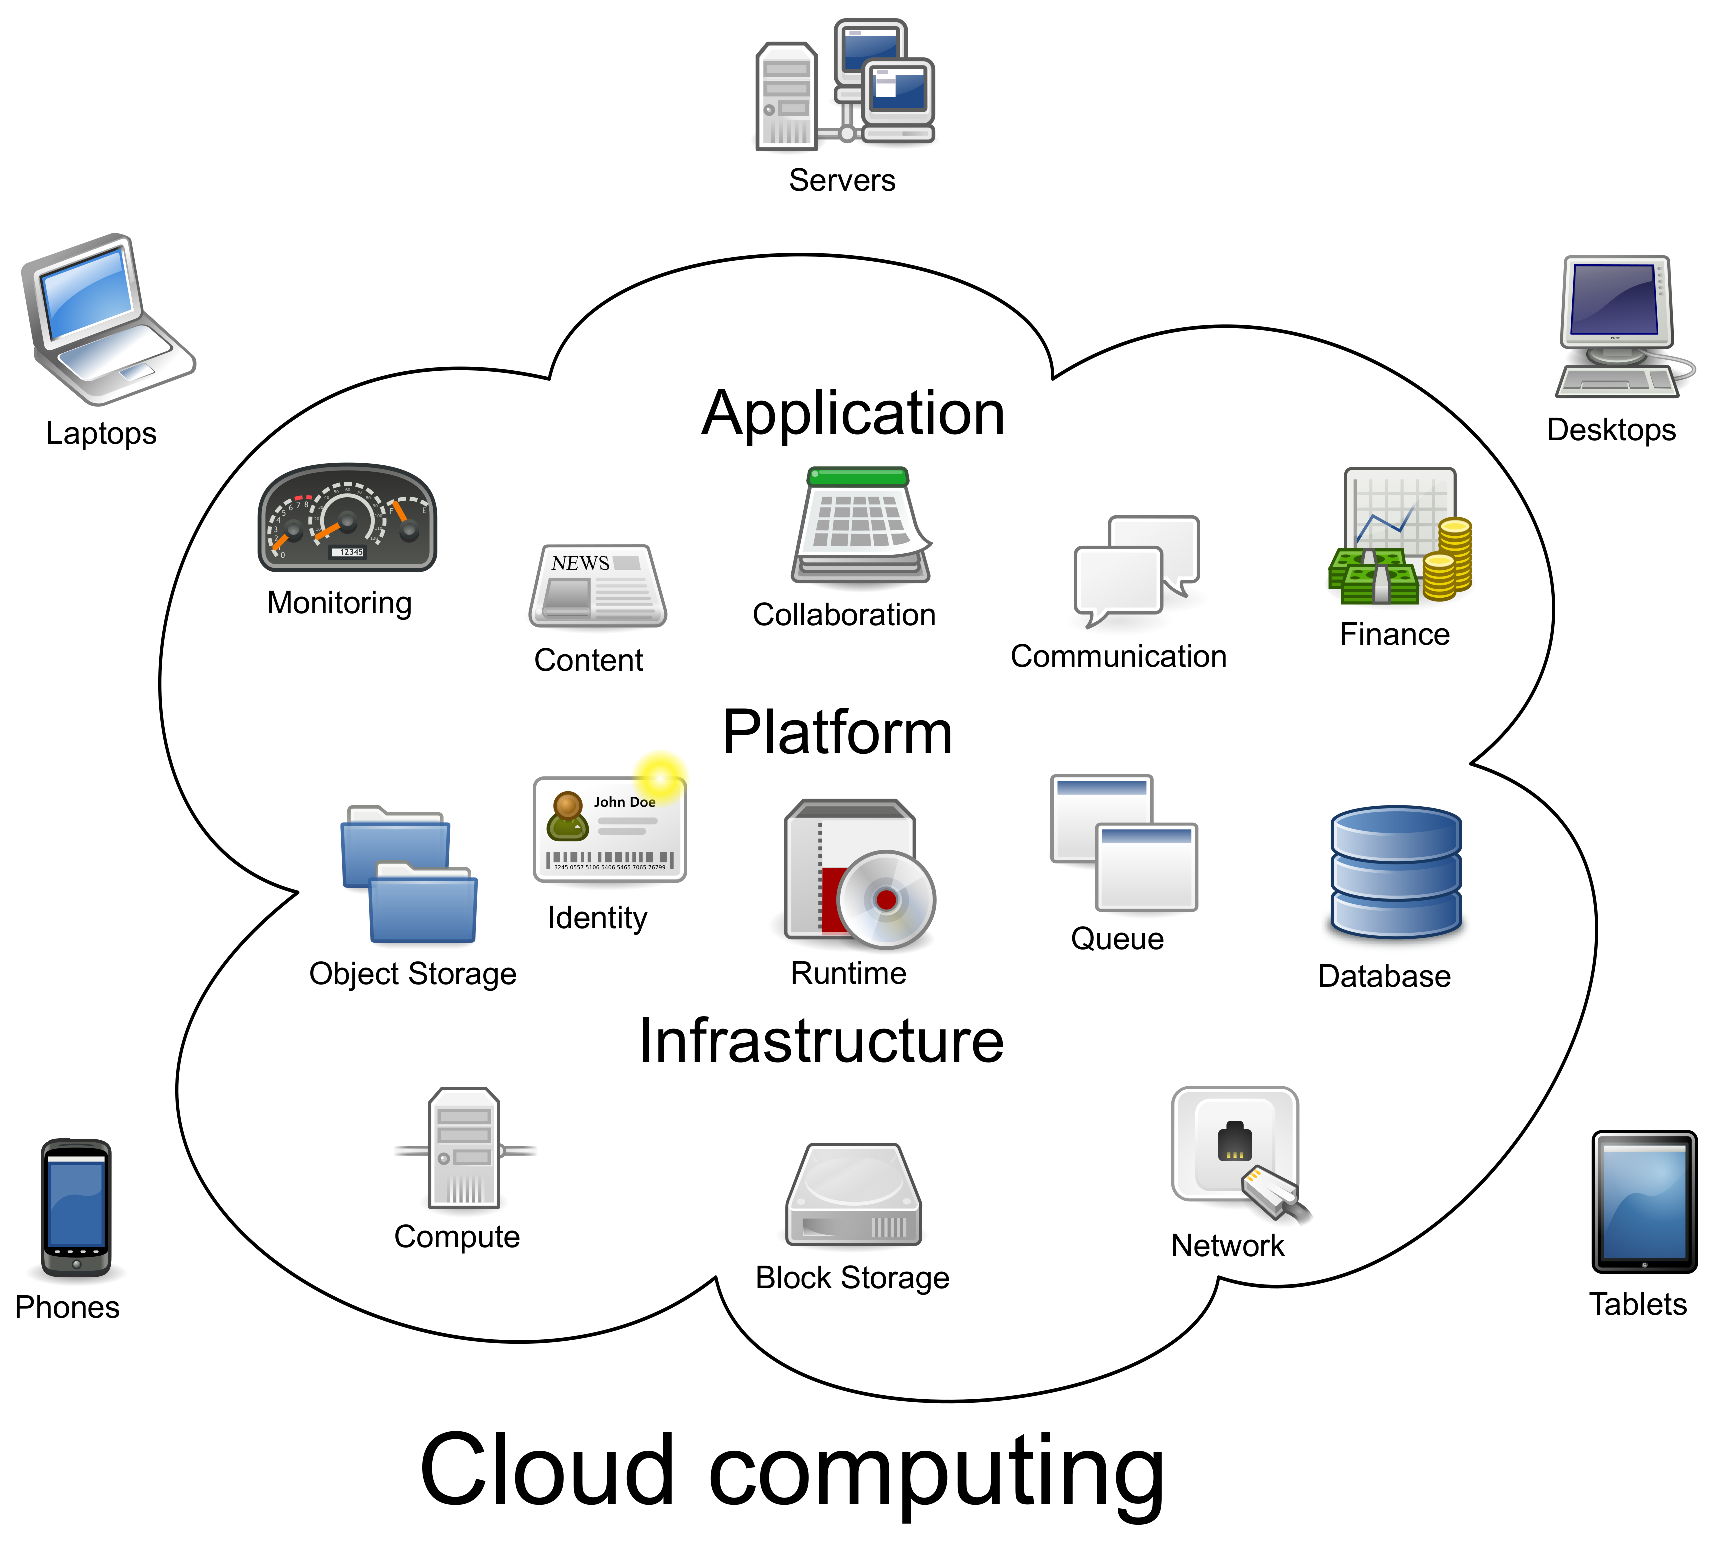
\includegraphics[scale=0.40]{imagens/cloud_computing.eps}
  \caption{Arquitetura Básica de Computação em Nuvem\cite{cloudcomputing}}
\end{figure}

Essas mudanças de paradigma motivaram a criação e consolidação do que conhecemos hoje como Computação em Nuvem, área fortalecida e necessária no desenvolvimento de programas modernos. Ao longo dos pŕoximos capítulos, haverá a explanação em detalhes de como funciona uma arquitetura em nuvem básica, seus desafios técnicos e as principais soluções existentes no mercado.

\chapter{Histórico}
\capepigrafe[0.5\textwidth]{I don't need a hard disk in my computer if I can get to the server faster... carrying around these non-connected computers is byzantine by comparison.}{Steve Jobs\cite{quotes}}

\section{Contexto}

\nocite{precloudcomputing}
A computação, em meados dos anos 90, consistia na evolução do computador pessoal e na consolidação da internet pelo mundo todo. A essência das aplicações construídas estava na distribuição de programas pela internet. Com o advento de aplicações web, torna-se necessário hospedar essas aplicações em servidores. Geralmente, era uma máquina física dedicada ao serviço, onde a aplicação ficaria hospedada, recebendo suas requisições.

\section{Problemas}

No contexto da época, esses servidores dedicados falhavam com certa frequência. Em casos de falha, o administrador do sistema precisava colocar uma nova máquina para atender a demanda, enquanto entendia a falha de \textit{software} ocorrida. Porém, toda a provisão de novos servidores para gerar redundância e tolerância a falhas aumentava a probabilidade de máquinas físicas falharem, gerando maiores problemas e dificuldades para manutenção.

\section{Primórdios}


Em 2006, a Amazon, percebendo a oportunidade de diversificar seu negócio atuando com provisionamento de infraestrutura, gerenciando máquinas ociosas de acordo com os horários possíveis e cuidando de toda a manutenção trabalhosa pelo lado do desenvolvedor, formulou e lançou a primeira versão do Amazon Elastic Compute Cloud (EC2), o primeiro produto voltado para a computação em nuvem, com o propósito de atender essa necessidade encontrada e vender infraestrutura para o usuário final.

\begin{figure}[h!]
  \centering
  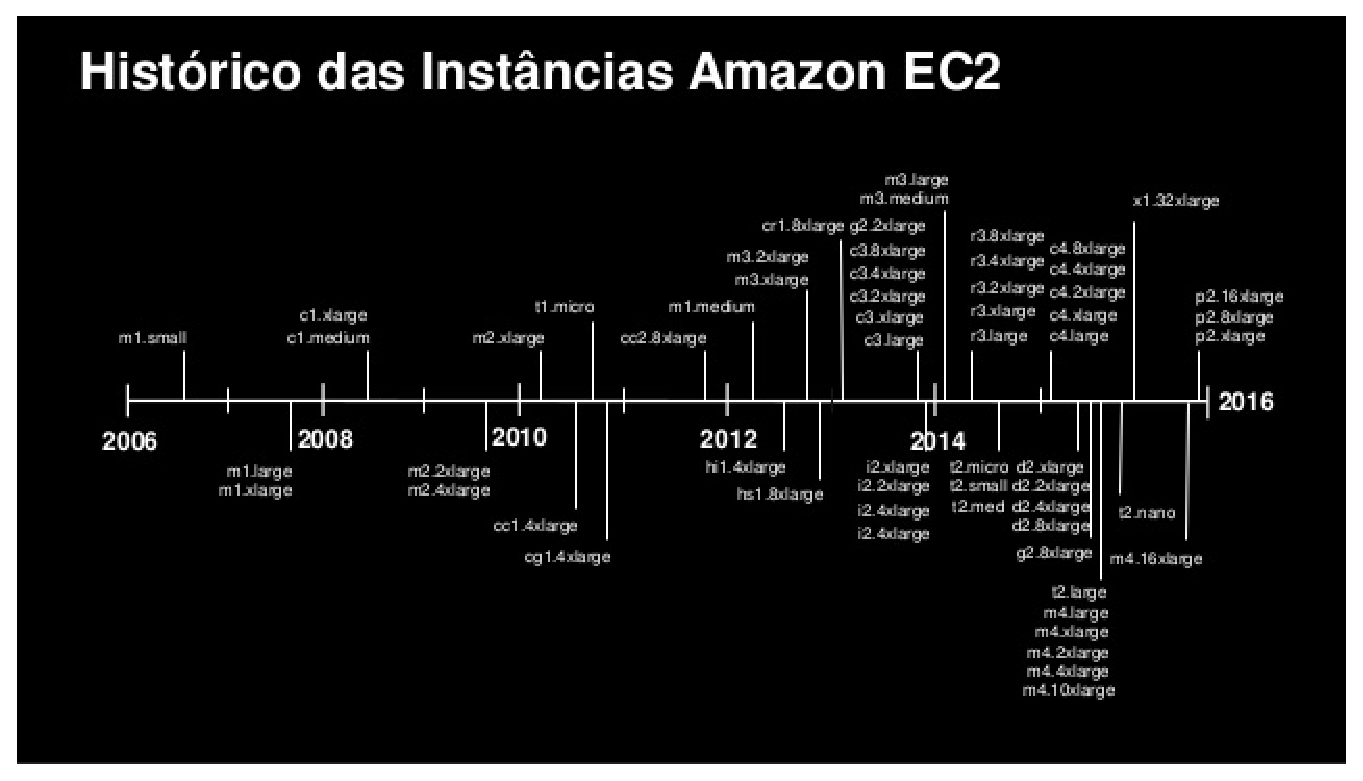
\includegraphics[scale=0.60]{imagens/ec2_history.eps}
  \caption{Histórico do Amazon EC2\cite{ec2history}}
\end{figure}

A postagem original no site da Amazon anunciava o serviço (em inglês)\cite{postamazonec2}:

\begin{citacaoLonga}
  Amazon Elastic Compute Cloud (Amazon EC2) is a web service that provides resizable compute capacity in the cloud. It is designed to make web-scale computing easier for developers. Just as Amazon Simple Storage Service (Amazon S3) enables storage in the cloud, Amazon EC2 enables “compute” in the cloud. Amazon EC2’s simple web service interface allows you to obtain and configure capacity with minimal friction. It provides you with complete control of your computing resources and lets you run on Amazon’s proven computing environment. Amazon EC2 reduces the time required to obtain and boot new server instances to minutes, allowing you to quickly scale capacity, both up and down, as your computing requirements change. Amazon EC2 changes the economics of computing by allowing you to pay only for capacity that you actually use.
\end{citacaoLonga}

\section{Impactos}

Essencialmente, a Amazon comercializou o conceito de infraestrutura como serviço (\textit{IaaS}). A revolução iniciada na época permitiu que muitas aplicações hospedadas em servidores físicos fossem migrados para a infraestrutura da Amazon. A cobrança realizada por hora de instância virtual carregada era bem inferior aos custos (tanto reais quanto de trabalho) de manter uma infraestrutura física equivalente, fora o fato de que a ociosidade foi drasticamente reduzida, pois o gerenciamento inteligente do EC2 permitia que uma mesma máquina atendesse dois serviços em horários distintos.

\begin{figure}[h!]
  \centering
  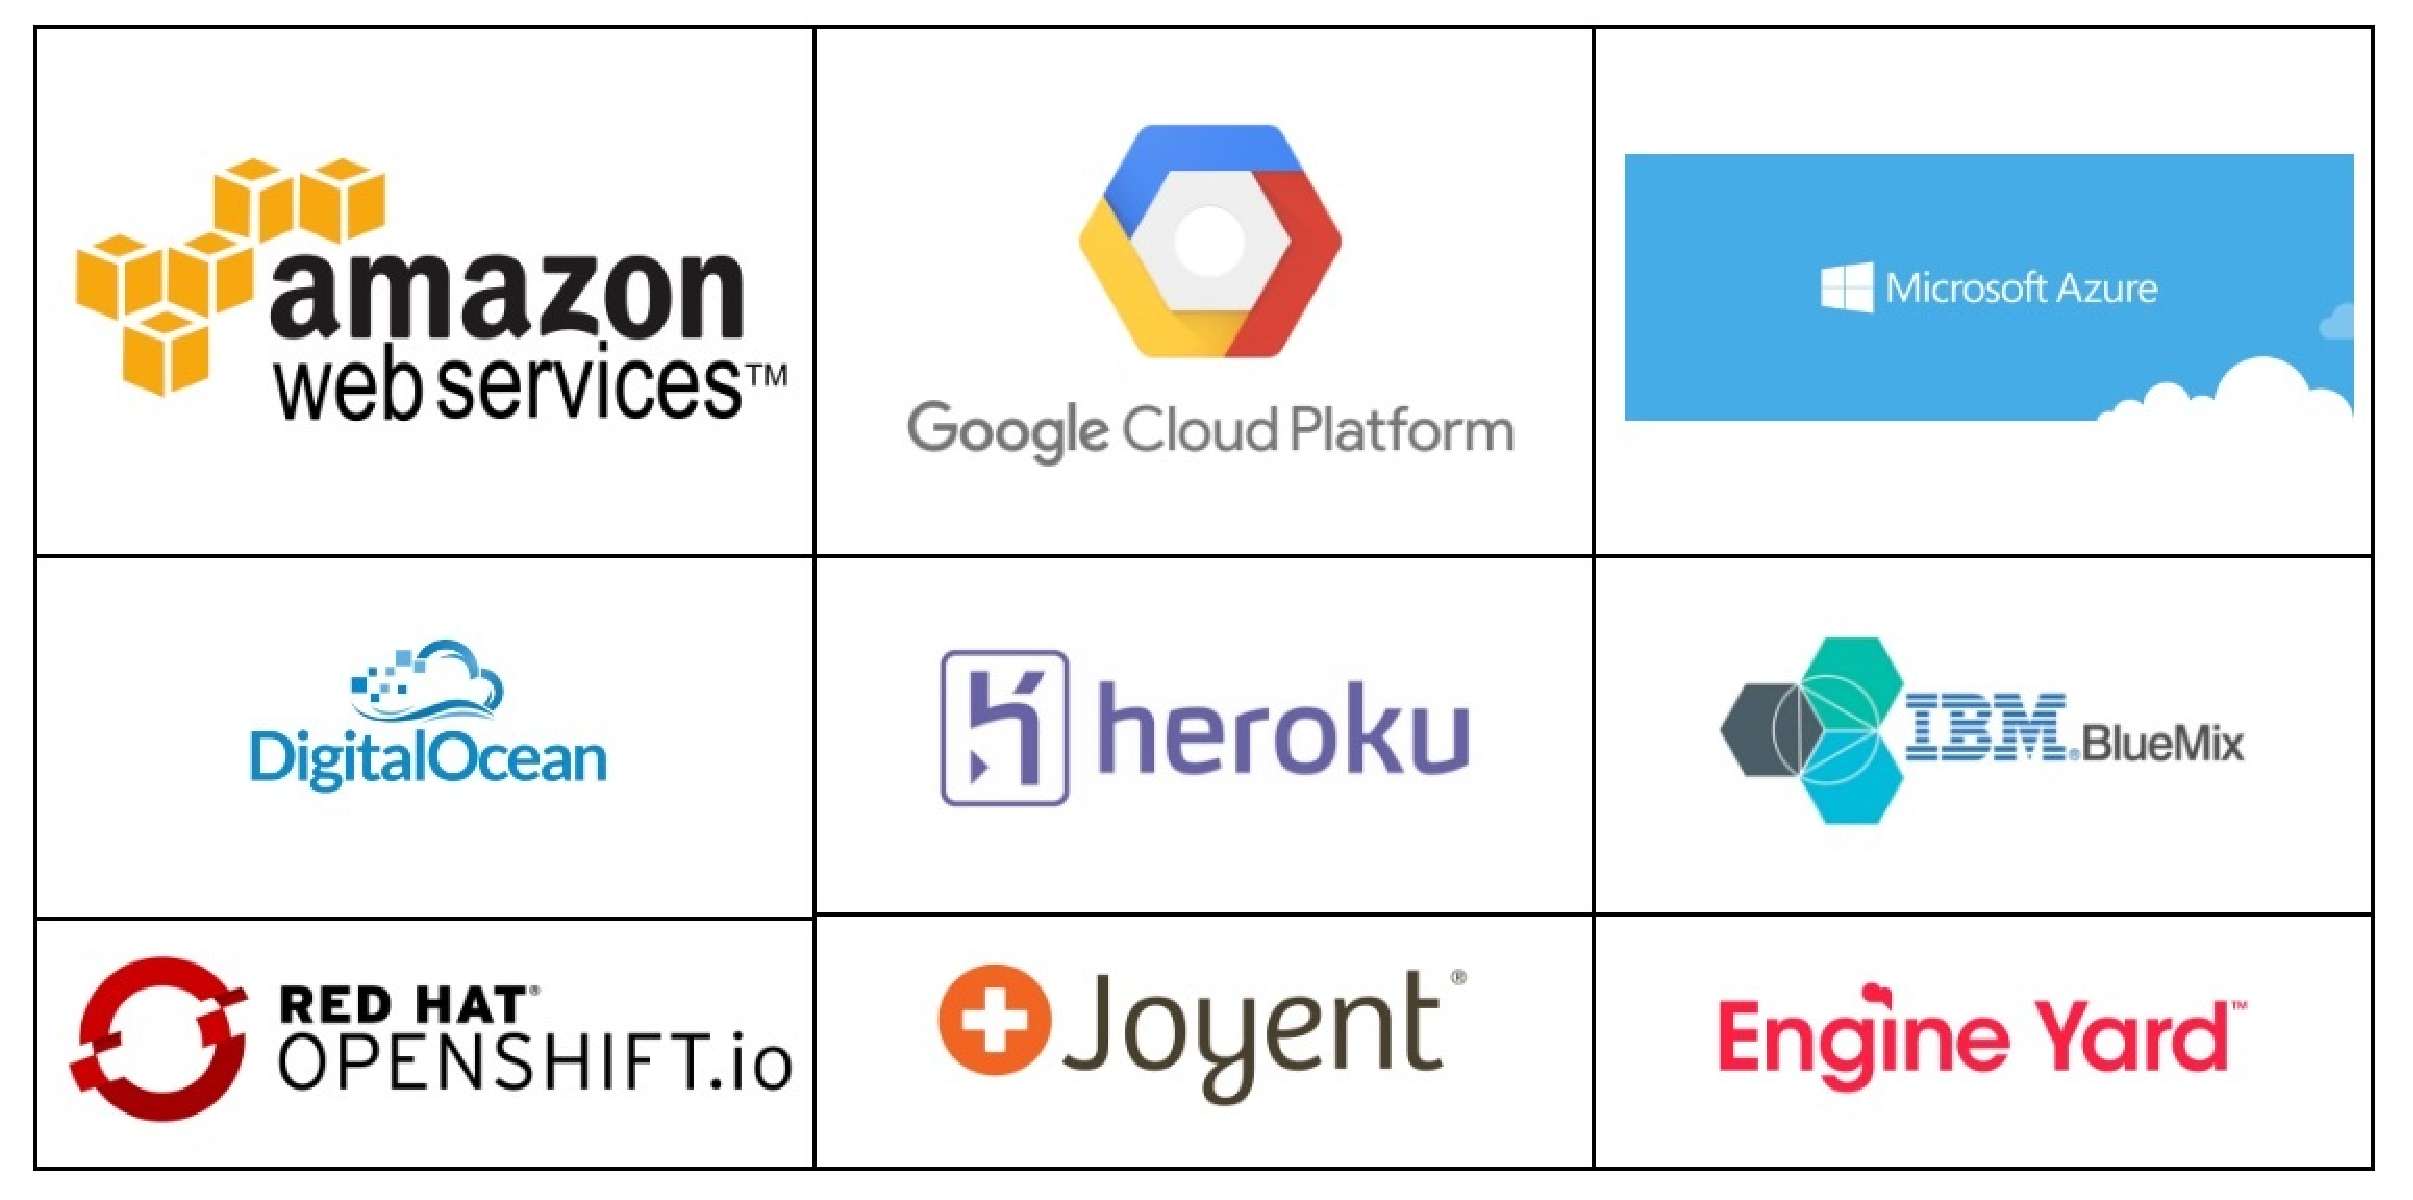
\includegraphics[scale=0.40]{imagens/clouds.eps}
  \caption{Algumas soluções de Computação em Nuvem\cite{clouds}}
\end{figure}

Com o trunfo do EC2, outras soluções ganharam força, merecendo destaque para: \textbf{Salesforce Heroku}, \textbf{Google Cloud} e \textbf{Microsoft Azure}, que serão exploradas adiante.


\part{Aspectos Conceituais}

\chapter{Conceitos básicos}
%Basic cloud definitions
Este capítulo introduz as definições e os conceitos básicos quando se trata de Cloud Computing.

\section{Definição de Cloud Computing}
	Computação em Nuvem (do Inglês \textit{Cloud Computing}) é segundo a NIST (\textit{National Institute of Standards and Technology}) um modelo para prover um acesso de rede a um grupo compartilhado (\textit{shared pool}) de recursos computacionais (recursos como capacidade de rede, servidores, armazenamento, aplicações e serviços) de forma ubíqua, prática e sob demanda.

	Tal acesso deve ser rapidamente provisionado e lançado com o mínimo de gerenciamento e interação com o provedor de serviços por parte da aplicação.

	O modelo de computação em nuvem deve possuir algumas características básicas, que estão descritas na secção seguinte.

\section{Características básicas de Cloud Computing}
	A NIST define 5 características essenciais do modelo de Cloud Computing:
	\begin{itemize}
		\item
			Serviço sobre demanda: Um consumidor pode provisionar unilateralmente capacidades computacionais, como tempo de servidor e armazenamento de rede, conforme for necessário, sem qualquer interação humana com o provedor de serviço;
		\item
			Agrupamento de recursos: Os recursos de computação do provedor são agrupados para atender a vários consumidores usando um modelo "multi inquilino", com diferentes recursos físicos e virtuais dinamicamente
			atribuídos e reatribuídos de acordo com a demanda do consumidor. Existe uma sensação de independência de localização pois o cliente geralmente não tem controle ou conhecimento sobre a localização exata dos recursos fornecidos, mas pode ser capaz de especificar a localização em um nível
			abstração (por exemplo, país, estado ou datacenter). Exemplos de recursos incluem armazenamento, processamento, memória e largura de banda de rede.
		\item
			Amplo acesso à rede: Os recursos estão disponíveis na rede e são acessados por meio de mecanismos que promovam o uso por plataformas heterogêneas por clientes em diversos dispositivos (por exemplo, telefones celulares, tablets, laptops e estações de trabalho). Esta característica promove o conceito de computação ubíqua, isto é, em toda parte, onipresente.
		\item
			Elasticidade rápida: Os recursos podem ser provisionados e liberados elasticamente, em alguns casos automaticamente, proporcionando uma escalabilidade crescente ou descrescente conforme a demanda. Os recursos disponíveis normalmente aparentam ser ilimitados para o consumidor, podendo ser requisitidados em qualquer quantidade e a qualquer momento.
		\item
			Serviço mensurável: Os sistemas em nuvem controlam e otimizam automaticamente o uso de recursos, aproveitando-se de uma capacidade de medição em um nível de abstração apropriado ao tipo de serviço (por exemplo, armazenamento, processamento, largura de banda e contas de usuário ativas). O uso de recursos pode ser monitorado, controlado e reportado, gerando transparência tanto para o fornecedor e consumidor do serviço utilizado.
	\end{itemize}


\chapter{Modelos para Cloud Computing}
	Este capítulo introduz brevemente os modelos de serviço de cloud computing que podem ser adotados por um provedor e os modelos de \textit{deployment}, nas secções seguintes.

\section{Modelos de serviços}
	A teoria por trás dos serviços de computação em nuvem abrange três elementos principais: software, plataforma e infraestrutura. Temos os seguintes modelos de serviço:

	\begin{itemize}
		\item
			\textbf{SaaS, Software as a Service} ("Software como um serviço") 

			Neste modelo é oferecido ao consumidor o uso de aplicações de um provedor que rodam sobre uma infraestrutura em nuvem. Estas aplicações são acessíveis a partir de vários dispositivos clientes por meio de uma interface simples, como um navegador da web, ou uma interface de por meio de um programa (mobile ou desktop). 

			O consumidor não gerencia ou controla a infraestrutura de nuvem por trás da aplicação, incluindo rede, servidores, sistemas operacionais, armazenamento ou capacidade da aplicação individual. São disponibilizadas apenas configurações do aplicativo específicas para aquele usuário individual.

			Alguns exemplos de SaaS são serviços de \textit{webmail}, \textit{streaming} de vídeos, conversão de arquivos e trabalho colaborativo com arquivos. Este modelo não será mais detalhado neste trabalho.

		\item
			\textbf{PaaS, Platform as a Service} ("Plataforma como um serviço") 

			A capacidade fornecida ao consumidor é de implantar na nuvem aplicações criadas por meio de linguagens de programação, bibliotecas, serviços e ferramentas suportadas pelo provedor. Tais aplicações podem ser criadas pelo próprio consumidor, ou consumidas por este.

			Assim como no modelo de SaaS, o consumidor geralmente não gerencia ou têm controle sobre a infraestrutura de nuvem por trás, incluindo rede, servidores, sistemas operacionais, ou armazenamento. Porém o consumidor as tem controle sobre os aplicativos implantados e possivelmente sobre definições de configuração para o ambiente de hospedagem do aplicativo.

			Como exemplos de provedores no mercado temos \textit{IBM Bluemix}, \textit{Heroku}, e \textit{Windows Azure Cloud}.
		\item
			\textbf{IaaS, Infrastructure as a Service} ("Infraestrutura como um serviço") 

			A capacidade oferecida ao consumidor é provisionar processamento, armazenamento, redes e outros recursos fundamentais de computação onde o consumidor é capaz de implantar e executar software arbitrário, incluindo-se sistemas e aplicações. O consumidor não gerencia nem controla a infraestrutura de nuvem por trás, mas tem controle sobre sistemas operacionais, armazenamento e aplicativos implantados. Possivelmente possui também um controle limitado de componentes de rede (por exemplo, firewalls de host). Geralmente acompanha serviços de máquinas virtualizadas.

			Alguns exemplos de provedores no mercado são \textit{Amazon Web Services}, \textit{Microsoft Azure}, \textit{Google Cloud} e \textit{VMware Cloud on AWS}. 
	\end{itemize}

\section{Modelos de implantação}
	Os modelos de implantação (\textit{deployment models}) a seguir delimitam as formas possíveis de tarifação dos serviços, as possíveis localizações da infraestrutura física e o público de escopo. São eles:

	\begin{itemize}
		\item
			\textbf{Nuvem privada}: A infraestrutura de nuvem é disponibilizada para uso exclusivo por uma única organização, compreendendo vários consumidores (\textit{business units}). Pode ser propriedade e gerenciada pela própria organização, um terceiro ou alguma combinação de ambos, e pode existir dentro ou fora das instalações da organização.
		\item
			\textbf{Nuvem comunitária}: A infraestrutura em nuvem é de uso exclusivo por uma comunidade de consumidores de organizações que compartilham mesmos interesses (por exemplo, missão, requisitos de segurança, políticas e considerações de conformidade). Pode ser de propriedade e administrada por uma ou mais organizações da comunidade, um terceiro, ou alguma combinação de ambos, e pode existir dentro ou fora das instalações.
		\item
			\textbf{Nuvem pública}: A infraestrutura de nuvem é para o uso aberto pelo público em geral. Pode ser propriedade ou gerenciada por uma organização comercial, acadêmica ou governamental, ou alguma combinação destes. Existe dentro das instalações do provedor de nuvem.
		\item
			\textbf{Nuvem híbrida}: A infraestrutura de nuvem é uma composição de duas ou mais infraestruturas de nuvens distintas (privadas, comunitárias ou públicas) que permanecem como entidades únicas, mas unidas por tecnologia padronizada ou proprietária permitindo portabilidade de dados e aplicações (por exemplo, \textit{cloud bursting} para balanceamento de carga entre nuvens).
	\end{itemize}


\chapter{Arquitetura}
	Este capítulo apresenta uma arquitetura de referência para cloud computing na primeira secção. Na secção final apresenta boas práticas e métodos para arquitetar uma aplicação que deve ser colocada em um ambiente de nuvem.

\section{Arquitetura de referência}
	O objetivo da arquitetura de referência apresentada a seguir é de providenciar uma taxonomia simples e sem ambiguidade para os três modelos de serviço:
	\begin{itemize}
		\item
			Software as a Service (SaaS)
		\item
			Platform as a Service (PaaS)
		\item
			Infrastructure as a Service (IaaS)
	\end{itemize}

	Tal arquitetura deve disponibilizar uma visão unificada das cinco características essenciais da NIST:
	\begin{itemize}
		\item
			Serviço sobre demanda
		\item
			Amplo acesso à rede
		\item
			Agrupamento de recursos
		\item
			Elasticidade rápida (escalabilidade)
		\item
			Serviço mensurável
	\end{itemize}

	Após pesquisar informações disponibilizadas por provedores, instituições de pesquisa e de consultoria na área achamos interessante a seguinte arquitetura de referência:

	\begin{figure}[h!]
  	\centering
  	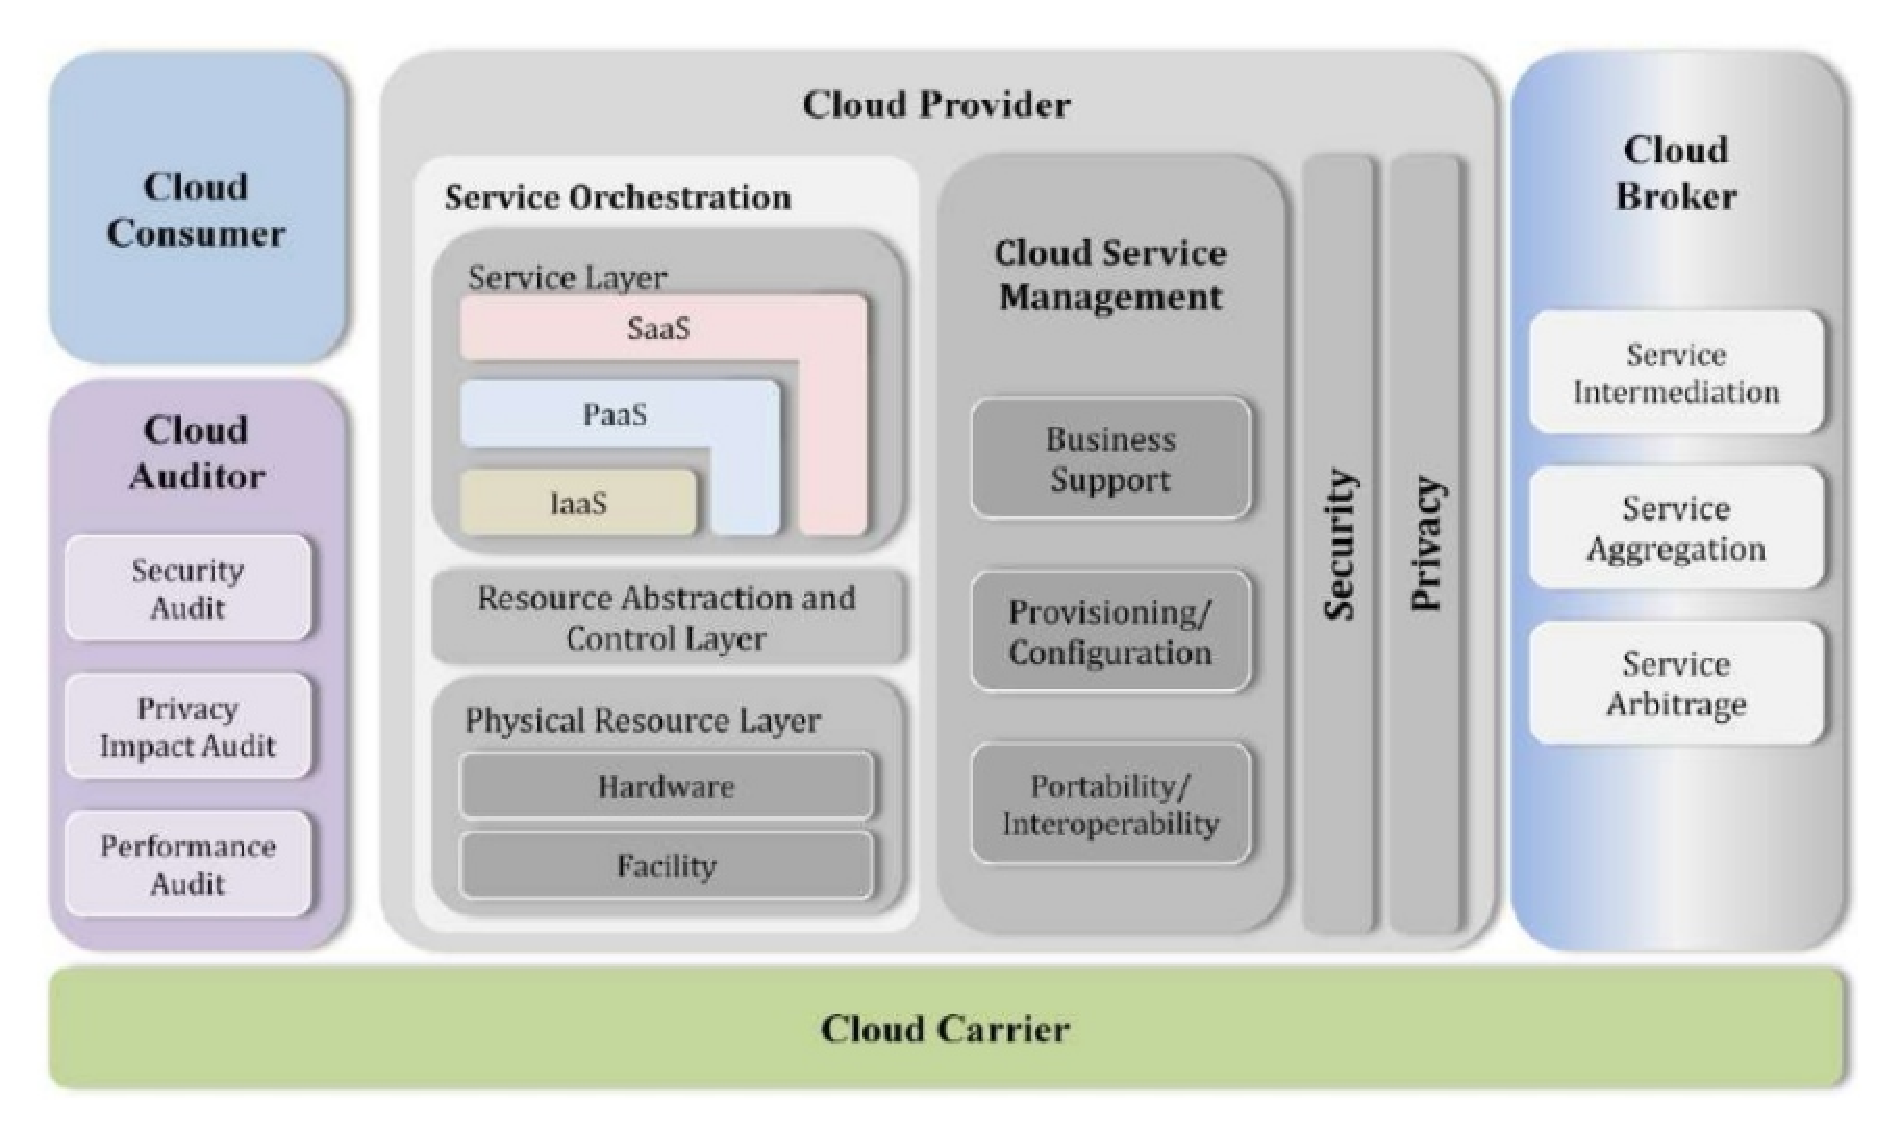
\includegraphics[scale=0.5]{imagens/cloudarch.eps}
  	\caption{Arquitetura de referência para Cloud Computing}
	\end{figure}

	\subsection{Cloud Consumer}
	Representa classes de consumidores para cada modelo possível de serviço. 

	No caso de SaaS são diversos departamentos operacionais de uma empresa, consumindo serviços de ERP, CRM, vendas, finanças, RH, redes sociais, webmail etc. 

	No caso de PaaS são os setores de análise de dados e desenvolvimento, que consomem serviços de BI, banco de dados, \textit{deployment} de aplicações, integração de sistemas e desenvolvimento e testes.

	Por fim, os consumidores de IaaS são os setores da empresa responsável pela infraestrutura e IT, que consomem serviços de backup e recuperação, gerenciamento de serviços, armazenamento, hospedagem de plataformas etc.

	\subsection{Cloud Auditor}
	Cloud Auditor é o componente responsável por relatar e registrar as ações relativas a segurança, privacidade e performance da nuvem, tanto para fins de transparência para os consumidores quanto de regulamentação governamental para rastrear atividades suspeitas e irregulares. Pode ser tanto um órgão governamental ou uma entidade fiscalizadora global na Internet.

	\subsection{Cloud Provider}
	Cloud Provider é o provedor de nuvem como a \textit{Amazon Web Services}, \textit{Microsoft Azure}, \textit{Netflix}, \textit{Youtube}, dentre outros. Dependendo das categorias de modelo de serviço em que o provedor se encaixa, ele poderá ter camadas de serviço de SaaS, PaaS ou IaaS. 

	As principais atividades do Cloud Provider são a implantação de serviços, a orquestração de serviços, o gerenciamento de serviços, a segurança e por fim, a privacidade. Deve gerenciar e abstrair toda lógica de controle e a camada física de recursos de hardware, bem como as instalações e locais físicos.

	\subsection{Cloud Broker}
	O Cloud Broker é responsável por uma espécie de serviço de corretagem. Este ator no ecossistema de nuvem é responsável por oferecer serviços de proteção jurídica durante a negociação de contratos com provedores de nuvem. 

	Oferece também serviços de diminuição de custos com o provedor, agregando diversos serviços a fim de obter o melhor custo-benefício.

	Por fim, pode oferecer serviços diferenciados, como um serviço adicional de segurança, para proteger o consumidor de vazamento de dados na nuvem.


	\subsection{Cloud Carrier}
	O Cloud Carrier são todas entidades responsáveis por disponibilizar a conexão e transporte de serviços na nuvem entre consumidores e provedores (Companhias de redes, telecomunicações, dispositivos de acesso e IoT). 

\part{Aspectos Técnicos}

\chapter{Estrutura}

\section{Hypervisor}
\section{Orquestrador}
\section{Armazenamento}
\section{Rede}

\chapter{Consideração técnicas sobre requisitos}
	Neste capítulo apresentamos algumas considerações técnicas e táticas para cumprir com êxito três principais requisitos não funcionais claros para Cloud Computing: disponibilidade, performance e segurança.

\section{Disponibilidade}

	Assume-se que a nuvem sempre estará disponível, 24 horas por dia, 7 dias por semana. Porém nenhum de seus componentes é a prova de falhas. O host físico de uma máquina virtual pode falhar, bem como a rede virtual com menor probabilidade, ao sofrer um ataque de negação de serviço (DDoS), por exemplo.

	Os provedores de serviço na nuvem fornecem dados aos consumidores sobre a porcentagem de tempo que a rede pode ficar disponível. Apesar de ser um número pequeno (para alguns planos de serviço da AWS variam entre 0,05\% e 0,001\%), é de responsabilidade do arquiteto do sistema que consumidor projetá-lo de tal forma que seja incluído um plano de contingência para essa indisponibilidade.

	Discutiremos algumas táticas a seguir:

	\subsection{Stateless}
	Arquitear sistemas \textit{stateless} (Sem estado) permite que qualquer instância de serviço possa servir igualmente uma requisição do cliente. Assim, se um servidor falha as requisições são redirecionadas para outra instância de serviço.

	\subsection{Instâncias reservas}
	O sistema deve incluir instâncias reservas da aplicação, para onde o tráfego de rede será redirecionado caso as instâncias principais venham a falhar.

	\subsection{Dados em zonas distintas}
	Um provedor na nuvem pode disponibilizar zonas distintas, que correspondem a \textit{data centers} distintos. O sistema então pode implementar uma redundância com diversas cópias dos dados espalhados por essas zonas. Se a rede de uma zona cair, uma zona que está ociosa ou a mais próxima ativa assume seu lugar.
	
	\subsection{Degradação silenciosa}
 	Os princípios para lidar com falhas em aplicações se baseam em táticas de renovação ou remoção de serviços:
	
	\begin{itemize}
	\item
	\textbf{Restauração rápida}:
	Crie \textit{timeouts} curtos para testar periodicamente o status de cada componente, restabelencendo-o antes que o sistema sinta essa falha.

	\item
	\textbf{Downgrades}:
	Cada feature é projetada com capacidade de ser degradada ou reduzida para uma representação de menor qualidade. Ex.: \textit{streaming} de vídeos.

	\item
	\textbf{Remoção de features}:
	Se a rede estiver mais lenta que o normal e a \textit{feature} não for crítica, ela deve ser removida da página.

	\end{itemize}
	\iffalse
	%TODO: Escrever
	\subsection{Exemplo: Netflix's Simian Army}

	\subsection{Exemplo: Skype Reverse NAT}
	\fi


\section{Performance}

Aplicações com boas performances computacionais são aquelas que respondem de forma instântanea ou com o tempo que lhe foi específicado, dentro de um limite tolerável que não prejudique uma atividade do usuário. Essa capacidade em uma máquina virtual ou física vai depender do que está sendo executado. Assim, cada aplicação deve monitorar a si mesma para determinar os recursos que recebe e quais irá precisar em um dado momento.

Uma vantagem da computação em nuvem é o provisonamento de \textit{hosts} elásticos, isto é, que permitem que recuroso adicionais sejam adquiridos conforme for necessário. Por meio do mecanismo de clusterização uma máquina virtual adicional pode provir essa capacidade computacional extra. Alguns provedores em nuvem alocam recursos automaticamente, enquanto outros consideram a alocação responsabilidade do usuário.

Mesmo se o provedor faça essa alocação de recursos de forma automática, a aplicação deve ser arquitetada de forma a estar ciente do uso de recursos atual e futuro, em qualquer instante de tempo. 

O provedor não pode fazer nada mais do que usar alguns algoritmos genéricos para determinar se há necessidade de alocar ou liberar mais recursos. Uma aplicação precisa ter um modelo de seu comportamento e estar preparada para fazer uma alocação sozinha de recursos. No pior caso, a aplicação pode comparar suas previsões com a do provedor para ter uma noção do que pode ocorrer.

\iffalse

\section{Segurança}
\fi

\part{Soluções do Mercado}

\chapter{Amazon Web Services}

\section{Introdução}
A Amazon Web Services (AWS) é uma plataforma de serviços em nuvem segura, oferecendo poder computacional, armazenamento de banco de dados, distribuição de conteúdo e outras funcionalidades para ajudar as empresas em seu dimensionamento e crescimento. Segundo pesquisas recentes \cite{rightscale}, é o provedor de nuvem que detém a maior parcela do mercado em termos de adoção, com aproximadamente 64\%. Sua gama de serviços é bastante ampla, como mostrado abaixo:

\begin{figure}[h!]
  \centering
  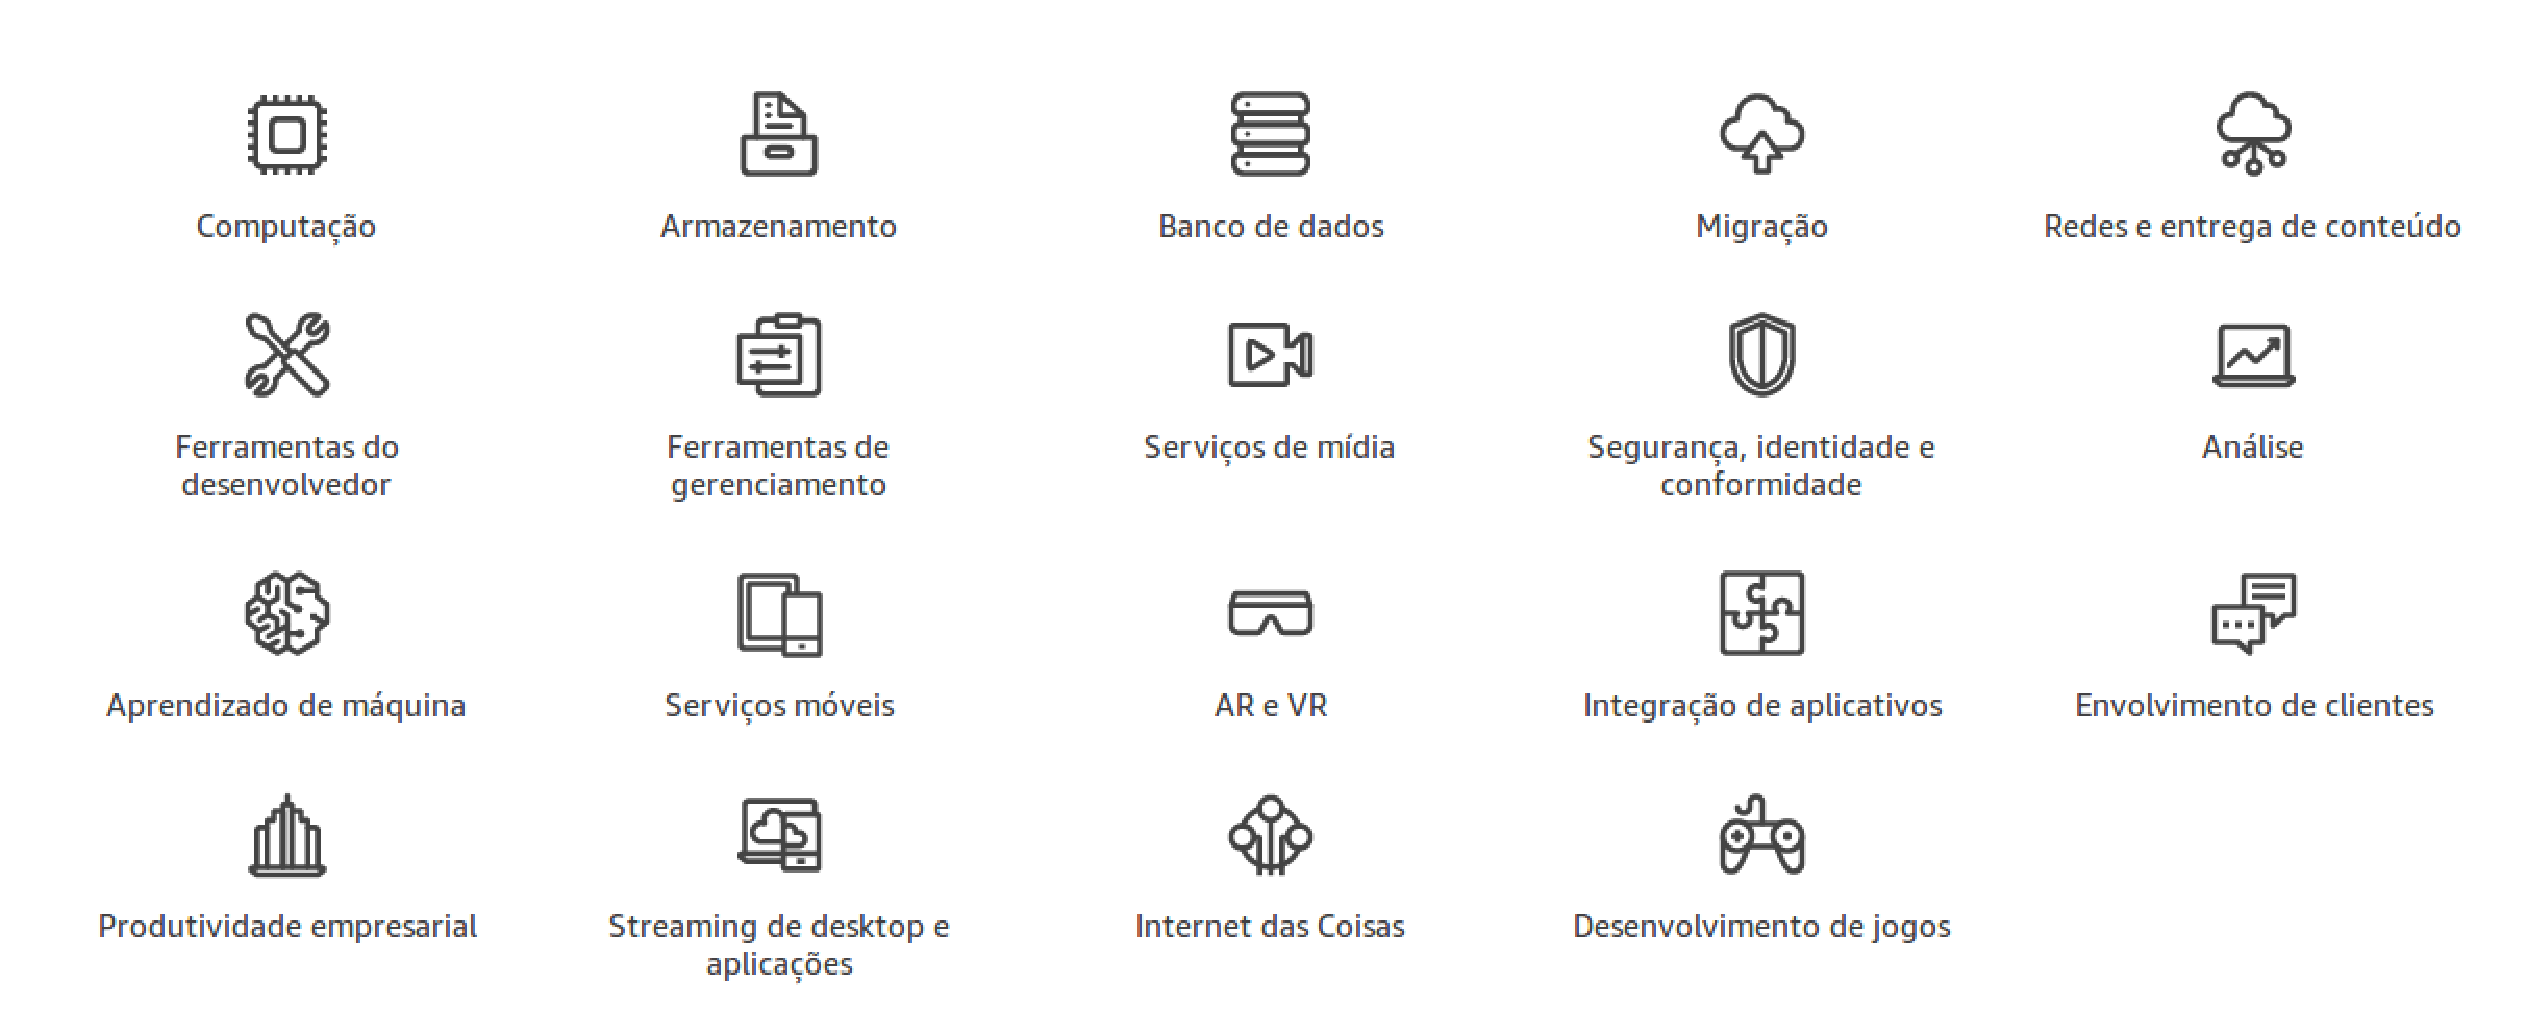
\includegraphics[scale=0.38]{imagens/aws-services.eps}
  \caption{Serviços da Amazon Web Services\cite{aws-services}}
\end{figure}

A AWS possui três serviços essenciais de nuvem para hospedagem de aplicações, sendo eles: \textbf{EC2}, \textbf{S3}, \textbf{RDS}. Além disso, possui soluções para outros variados campos da computação, como inteligência artificial, desenvolvimento \textit{mobile}, realidade virtual e internet das coisas.


\section{Funcionamento básico}
No contexto do documento, serão destacados os três serviços já citados anteriormente:


\begin{figure}[h!]
  \centering
  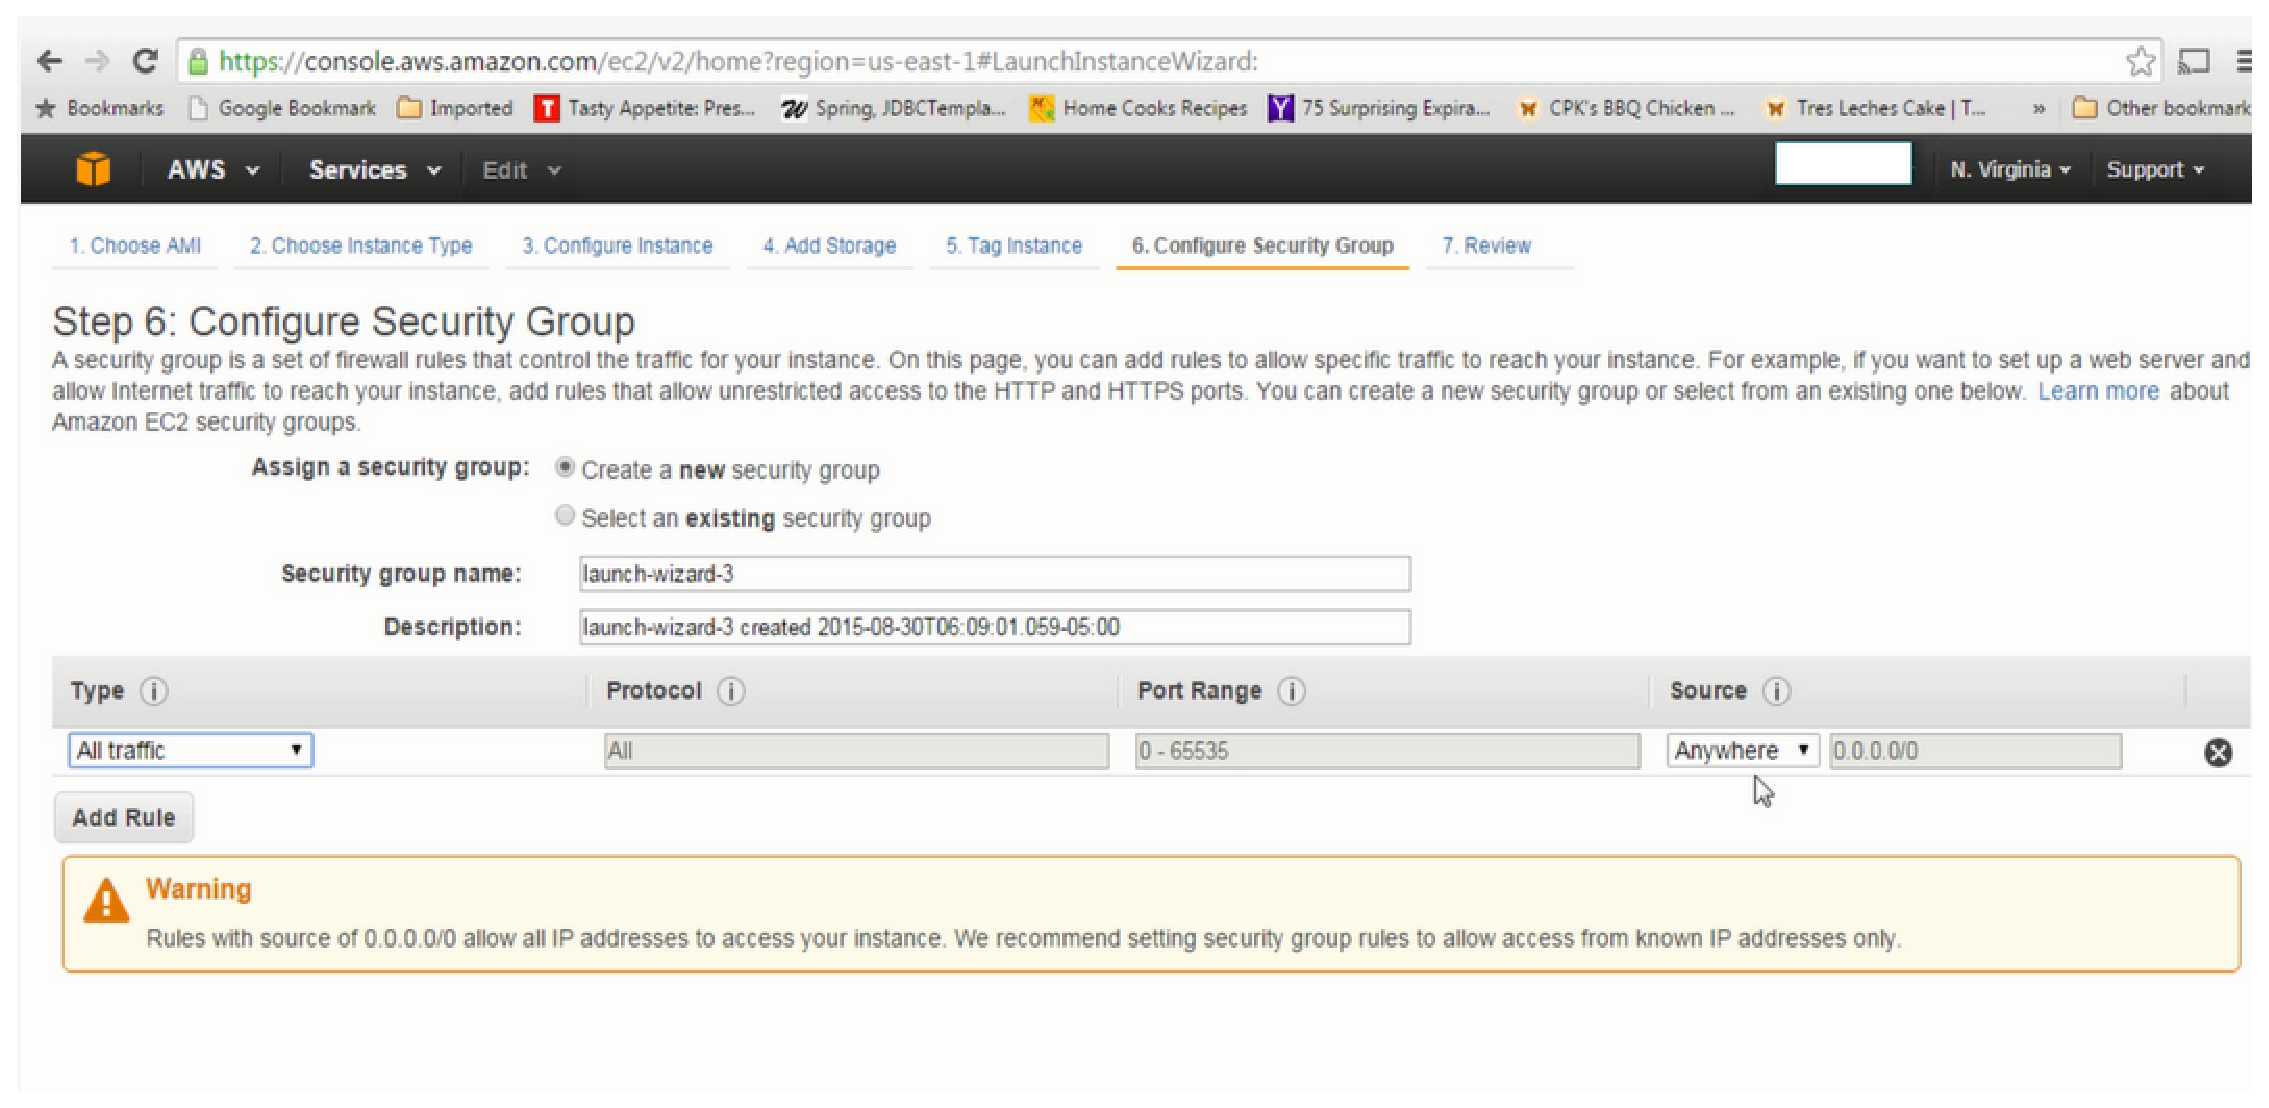
\includegraphics[scale=0.42]{imagens/aws-console.eps}
  \caption{Console da Amazon Web Services}
\end{figure}


\subsection{EC2}
O Amazon Elastic Compute Cloud (Amazon EC2) é o principal e mais básico serviço da AWS, e \textit{web} que disponibiliza capacidade computacional segura e redimensionável na nuvem. Ele foi criado para facilitar para os desenvolvedores a computação em nuvem na escala da \textit{web}. Possui várias \textit{features} bastante interessantes, com destaque para:
\begin{itemize}
  \item{\textbf{Elasticidade}: O Amazon EC2 permite aumento ou diminuição da capacidade em minutos em vez de horas ou dias. É possível contratar simultaneamente uma, centenas ou até milhares de instâncias de servidor. Também é possível usar o Amazon EC2 \textit{Auto Scaling} para manter a disponibilidade de frotas do EC2, além de ampliar e reduzir a escala dela, dependendo das necessidades específicas, com o objetivo de maximizar a performance e minimizar os custos;}
  \item{\textbf{Integração}: O serviço é integrado com uma séria de outros serviços da AWS, de maneira a prover um ambiente de computação em nuvem completo e seguro para uma série de possíveis aplicações do desenvolvedor;}
  \item{\textbf{Confiabilidade}: O EC2 oferece um ambiente altamente confiável, permitindo a contratação de instâncias de substituição de forma rápida e previsível. O serviço é executado dentro dos datacenters e da infraestrutura de rede comprovada da Amazon;}
  \item{\textbf{Baixo Custo}: Taxas são baixas e compatíveis com o poder computacional que realmente é utilizado pelo desenvolvedor.}
\end{itemize}

\subsection{S3}
O S3 (\textit{Simple Storage Service}) é o sistema de armazenamento da AWS. Segundo a definição da própria Amazon \cite{aws-s3}:

\begin{citacaoLonga}
Armazenamento de objetos para armazenar e recuperar qualquer quantidade de dados de qualquer local.
\end{citacaoLonga}

Possui bastante estabillidade e resiliência (compromisso de 99,999999999\% \cite{aws-s3}), visto que os dados são distribuídos automaticamente entre no mínimo três instalações físicas, separadas geograficamente dentro de uma região da AWS. Permite inclusive a replicação de dados entre as regiões da própria AWS.

É uma das soluções com maior porcentagem de adoção da Amazon, havendo inúmeros casos de sucesso de empresas grandes e com demandas bastante complexas. Cabe citar dois exemplos interessantes do mercado, e em áreas distintas: 
\begin{itemize}
  \item{\textit{\textbf{Netflix}}: empresa americana de \textit{streaming} de vídeo, disponibiliza bilhões de horas de conteúdo para clientes em todo o mundo atráves do S3. Além disso, usa o serviço como \textit{data lake} para suas soluções de \textit{big data}}.
  \item{\textit{\textbf{Airbnb}}: serviço online para que pessoas anunciem e reservem acomodações e meios de hospedagem. Utiliza o Amazon S3 para armazenar arquivos estatístcos e de \textit{backup}, além de mais de 10 Petabytes de fotografias de usuários e de acomodações.}
\end{itemize}

\subsection{RDS}

O Amazon RDS (\textit{Relational Database System}) é uma solução que fornece bancos de dados relacionais gerenciados, de maneira escalável e automatizando uma série de funções como administração, aplicação de \textit{patches} e \textit{backups}. Atualmente, trabalham com cinco dos principais mecanismos de bancos de dados SQL do mercado (tanto \textit{open source} como proprietários). São eles: 

\begin{itemize}
  \item{PostgreSQL}
  \item{MySQL}
  \item{MariaDB}
  \item{Oracle}
  \item{Microsoft SQL Server}
\end{itemize}

Além disso, possuem uma solução de banco de dados própria, o \textbf{Amazon Aurora}, que é compatível com o MariaDB e o PostgreSQL, e também roda nas instâncias do RDS. Conforme citado no próprio site da AWS \cite{aws-aurora}:

\begin{citacaoLonga}
O Aurora é até cinco vezes mais rápido que bancos de dados MySQL padrão e três vezes mais rápido que bancos de dados PostgreSQL padrão. O serviço oferece a segurança, a disponibilidade e a confiabilidade de bancos de dados comerciais por um décimo do custo.
\end{citacaoLonga}

\section{Outros Serviços}

Para representar a vasta gama de serviços em nuvem que a AWS apresenta, pode ser citada a \textbf{Amazon Alexa}, um serviço de voz e inteligência artificial que permite a construção de experências de voz naturais, promovendo um meio para que os clientes interajam com a tecnologia do dia a dia. A Alexa possui uma coleção bastante rica de ferramentas, \textit{APIs} e documentação que tornam seu desenvolvimento bem acessível.


\section{Conclusão}

A AWS não é a líder de mercado (em termos de adoção) de \textit{cloud computing} atoa. Apresenta soluções de qualidade em praticamente todos os campos da computação, desde áreas mais consolidads como hospedagem mais simples de aplicativos, como em campos mais de pesquisa como \textit{machine learning} e inteligência artificial. A única desvantagem que pode apresentar com relação aos seus concorrentes seria com relação ao custo dos serviços, porém acaba dependendo bastante do propósito e do \textit{budget} de cada empresa ou usuário.

\chapter{Google Cloud}

\section{Introdução}

\chapter{Heroku}

\section{Introdução}

\chapter{Azure}
% \capepigrafe[0.5\textwidth]{``Uma frase bem legal sobre o legado deixado''}{Autor da frase bem legal}

\section{Introdução}


% ========== Referências ==========
% --- IEEE ---
%	http://www.ctan.org/tex-archive/macros/latex/contrib/IEEEtran
%\bibliographystyle{IEEEbib}

% --- ABNT (requer ABNTeX 2) ---
%	http://www.ctan.org/tex-archive/macros/latex/contrib/abntex2
\bibliographystyle{abntex2-num}

\bibliography{refs}

% ========== Apêndices (opcional) ==========
\apendice

% ========== Anexos (opcional) ==========
\anexo

\end{document}
